\documentclass[10pt, conference, letterpaper]{IEEEtran}
\usepackage{cite}
\usepackage{amsmath,amssymb,amsfonts}
\usepackage{algorithmic}
\usepackage{graphicx}
\usepackage{textcomp}
\usepackage{xcolor}
\usepackage{hyperref}
\usepackage{booktabs}
\usepackage{multirow}
\usepackage{url}
\usepackage{algorithm}

\def\BibTeX{{\rm B\kern-.05em{\sc i\kern-.025em b}\kern-.08em
    T\kern-.1667em\lower.7ex\hbox{E}\kern-.125emX}}

\begin{document}

\title{Double-Blind PQC: A Practical Application-Layer Framework for Integrating NIST Post-Quantum Cryptography in Virtual Private Networks\\
}

\author{\IEEEauthorblockN{Name 1 \\ Name 2}
\IEEEauthorblockA{\textit{School of Computer Science \& Engineering} \\
\textit{Vellore Institute of Technology, Chennai Campus}}
}

\maketitle

\begin{abstract}
The ongoing development of quantum computing technology constitutes a significant threat to the security of contemporary public-key cryptographic protocols. All algorithms that are based on integer factorization (RSA) or problems related to elliptic curves and discrete logarithms, such as those used in cryptography, will be compromised in the future by large-scale quantum computers. The ``Store Now, Decrypt Later'' attack paradigm makes this threat a pressing concern for today's cryptographic security. In this paper, we introduce Double Blind PQC, a software framework for end-to-end VPN communications that utilizes NIST-standardized post-quantum algorithms. Our framework utilizes ML-KEM-768 (Kyber) for key encapsulation, ML-DSA-65 (Dilithium) for digital signature authentication, and AES-256-GCM for symmetric key encryption. An important contribution of this work is the deterministic Application Layer Fragmentation Wrapper, which overcomes the key challenge of transferring post-quantum key sizes over the UDP protocol, where the payload size often exceeds the MTU. We compare the performance of our framework against other widely used classical algorithms such as X25519, SECP256R1, RSA-3072, and Ed25519. ML-KEM-768 is shown to have key generation performance that consistently exceeds even elliptic curve-based algorithms, thus confirming the feasibility of post-quantum algorithms in the context of VPN communications.
\end{abstract}

\begin{IEEEkeywords}
Post-Quantum Cryptography, CRYSTALS-Kyber, CRYSTALS-Dilithium, SPHINCS+, Falcon, VPN, WireGuard, Network Security, Key Encapsulation Mechanism, Latency Evaluation, MTU Fragmentation
\end{IEEEkeywords}

\section{Introduction}

\subsection{The Quantum Threat Horizon}
The security of internet communications today is almost solely provided by public-key cryptography. Protocols such as SSL/TLS, IPsec, and other cryptographic standards have made the internet a safer place. All public-key cryptographic algorithms, however, will be easily broken by future quantum computers. Algorithms such as RSA, elliptic curves, Diffie-Hellman, and other variants of these algorithms will not survive the advent of large-scale quantum computers. The ``Store Now, Decrypt Later'' attack paradigm has made this threat a pressing concern for today's cryptographic security.

The IPsec, OpenVPN, TLS~1.3, and WireGuard protocols utilize session key negotiation using Elliptic Curve Cryptography, specifically using the X25519 elliptic curve \cite{hulsing2017pqwireguard}. These protocols derive their strength from the difficulty of solving an elliptic logarithm problem, which is also a problem of integer factorization, both of which cannot be solved in a reasonable time on a classical computer.

However, Shor's algorithm, discovered in 1994, completely turns these calculations on their head. A quantum computer, if sufficiently advanced, will be able to solve both integer factorization and elliptic logarithm problems in a polynomial time, thus making RSA, ECDHE, and other such protocols completely insecure.

Furthermore, Grover's algorithm provides a speedup of a quadratic time complexity to brute-force methods, meaning that if a quantum computer is utilized, the security level will be halved, making it a whole lot easier to break symmetric encryption protocols such as AES. This means that an AES-128 encryption, for example, will only be 64 bits secure if a quantum computer is utilized, thus making AES-256 a minimum necessity \cite{shim2025qtrustnet}.

The reason why we know that quantum computer attacks will be a certainty, not a probability, is because of SNDL, a model of attack utilized by nations and other well-heeled groups to intercept and store encrypted communications. This encrypted communication will be decrypted when a crypto-relevant quantum computer (CRQC) is eventually brought online. However, if we're considering communications that have a long period of time in which they remain confidential, such as government, military, financial, and medical communications, then we're running out of time, not when quantum computers arrive.

\subsection{NIST PQC Standardization and Strategic Context}
As a direct result of the quantum computer threat, NIST began a multi-year standardization project to determine a set of cryptographic algorithms that will be secure against quantum computer attacks, resistant to both classical and quantum attacks. The candidate algorithms, which include structured lattices, code-based, isogeny-based, and multivariate polynomial-based, were extensively tested through multiple rounds of public cryptanalysis.

The final step in this process was to select ML-KEM, which is based on the CRYSTALS-Kyber scheme, as a key encapsulation scheme, and ML-DSA, which is based on the CRYSTALS-Dilithium scheme, as a digital signature scheme. The ML-KEM and ML-DSA are both based on the Module Learning with Errors problem over polynomial lattices, which is a well-founded problem believed to be secure against quantum attacks.

Two other signature schemes, namely Falcon, which is a lattice-based signature scheme with compact signature sizes, and SPHINCS+, which is a hash-based signature scheme, were also standardized. The latter scheme is attractive in case lattice-based signature schemes are found to be vulnerable in future cryptanalytic advances. The Falcon signature scheme, on the other hand, is attractive in bandwidth-constrained environments. It is worth noting, however, that although SPHINCS+ offers a viable option in case lattice-based signature schemes are found to be vulnerable, its larger signature size and slower signature generation rate make it less attractive for network protocols. In practice, ML-DSA and Falcon are the two most viable signature schemes for VPN authentication.

\subsection{Architectural Transport Integration Hurdles}
The MLWE-based algorithms are known to be secure, but there are many architectural hurdles in incorporating these algorithms in existing network architectures. The existing VPN protocols are designed with small key sizes in mind, which are typical in classical elliptic curve-based protocols. For instance, in X25519, a public key is merely 32 bytes long. In contrast, in ML-KEM-768, a public key is 1,184 bytes long. In ML-DSA-65, a signature is over 3,000 bytes long.

The increased size of these payloads poses a number of problems in transport layer. When transmitted via UDP, the recommended transport for high-speed VPNs, payloads larger than the standard Ethernet MTU size of 1,500 bytes will require IP fragmentation. In the case of UDP, if any one packet is dropped during transmission, the entire datagram is silently discarded with no retransmission mechanism. Realistically speaking, this means that the simple integration of Post-Quantum Cryptography, or PQC, is not a viable option and can even prevent the creation of the VPN tunnel altogether \cite{shim2025qtrustnet}.

\section{Background and Literature Review}

\subsection{Post-Quantum WireGuard}
H\"ulsing et al. \cite{hulsing2017pqwireguard} first proposed PQ-WireGuard, one of the first efforts to integrate the VPN protocol with the benefits of post-quantum cryptography. They replaced the standard Diffie-Hellman key exchange, which is based on interactive curve operations, with a unidirectional KEM-based handshake. Through the use of formal verification tools, they proved the newly modified version of the VPN to be cryptographically sound. Nevertheless, the performance penalty during the handshake phase is significant. Due to the large sizes of the keys and ciphertexts used in the KEM-based handshake, the performance penalty is measurable compared to the original 32-byte X25519-based handshake.

\subsection{qTrustNet and Hardware-Based PQC Interfaces}
Shim et al. \cite{shim2025qtrustnet} took a different route with the design and implementation of the qTrustNet VPN architecture. They integrate the NIST PQC suite with the security benefits of hardware-based security primitives. They integrate the post-quantum-based key exchange directly into the transport endpoints of the WireGuard VPN, which is combined with the local storage security benefits of Physically Unclonable Functions (PUFs). PUFs tie the security material directly to the physical characteristics of the individual hardware devices. Their results show low latency operation with sustained throughput approaching 8.5~Gbps on 10GbE network interfaces. The architecture ensures robust security guarantees; however, due to its dependency on hardware components like PUF devices and kernel-level modifications of the WireGuard implementation, portability is a concern.

\subsection{Identifying the Application Layer Gap}
PQ-WireGuard and qTrustNet operate at either the kernel level or slightly above, necessitating modifications to the internal state machine of the WireGuard implementation or hardware support modules, respectively. Though these approaches are highly effective, they are difficult to port across a range of different operating systems and network configurations.

The Double-Blind PQC framework bridges this application layer gap by operating entirely in the application layer rather than in the kernel level or above as in the case of PQ-WireGuard and qTrustNet. Our system utilizes a standard userspace process rather than kernel modules or hardware support modules, sacrificing some throughput compared to kernel-level support in favor of portability across a range of different operating systems and configurations; the same code can operate on any system which has a Python interpreter available and access to the PQC libraries.

\section{Threat Model and Assumptions}
The following threat model is proposed, which represents a worst-case scenario for public internet communication under quantum-era conditions:

\begin{itemize}
    \item \textbf{Dolev-Yao Network Adversary}: The adversary has complete control over the network channel between the Initiator and Responder nodes. They can intercept, read, modify, delay, reorder, replay, or drop any UDP packet in transit.
    \item \textbf{Quantum Computing Capability}: The adversary either currently possesses or will eventually obtain access to a CRQC capable of running Shor's and Grover's algorithms. All recorded traffic is assumed to be vulnerable to future decryption.
    \item \textbf{Endpoint Integrity}: We assume that the VPN client endpoints themselves are uncompromised - free from malware, side-channel vulnerabilities, or physical tampering. The endpoints are treated as trusted platforms.
\end{itemize}

Within this threat model, we require that the protocol provide two properties: mutual authentication, to prevent man-in-the-middle attacks even against an active quantum-capable adversary, and forward secrecy, to prevent compromise of long-term keys being used to reveal past session keys. Both properties rely on the hardness of the MLWE problem against quantum algorithms.

\section{Cryptographic Foundation and Architecture}

\begin{figure}[!t]
\centering
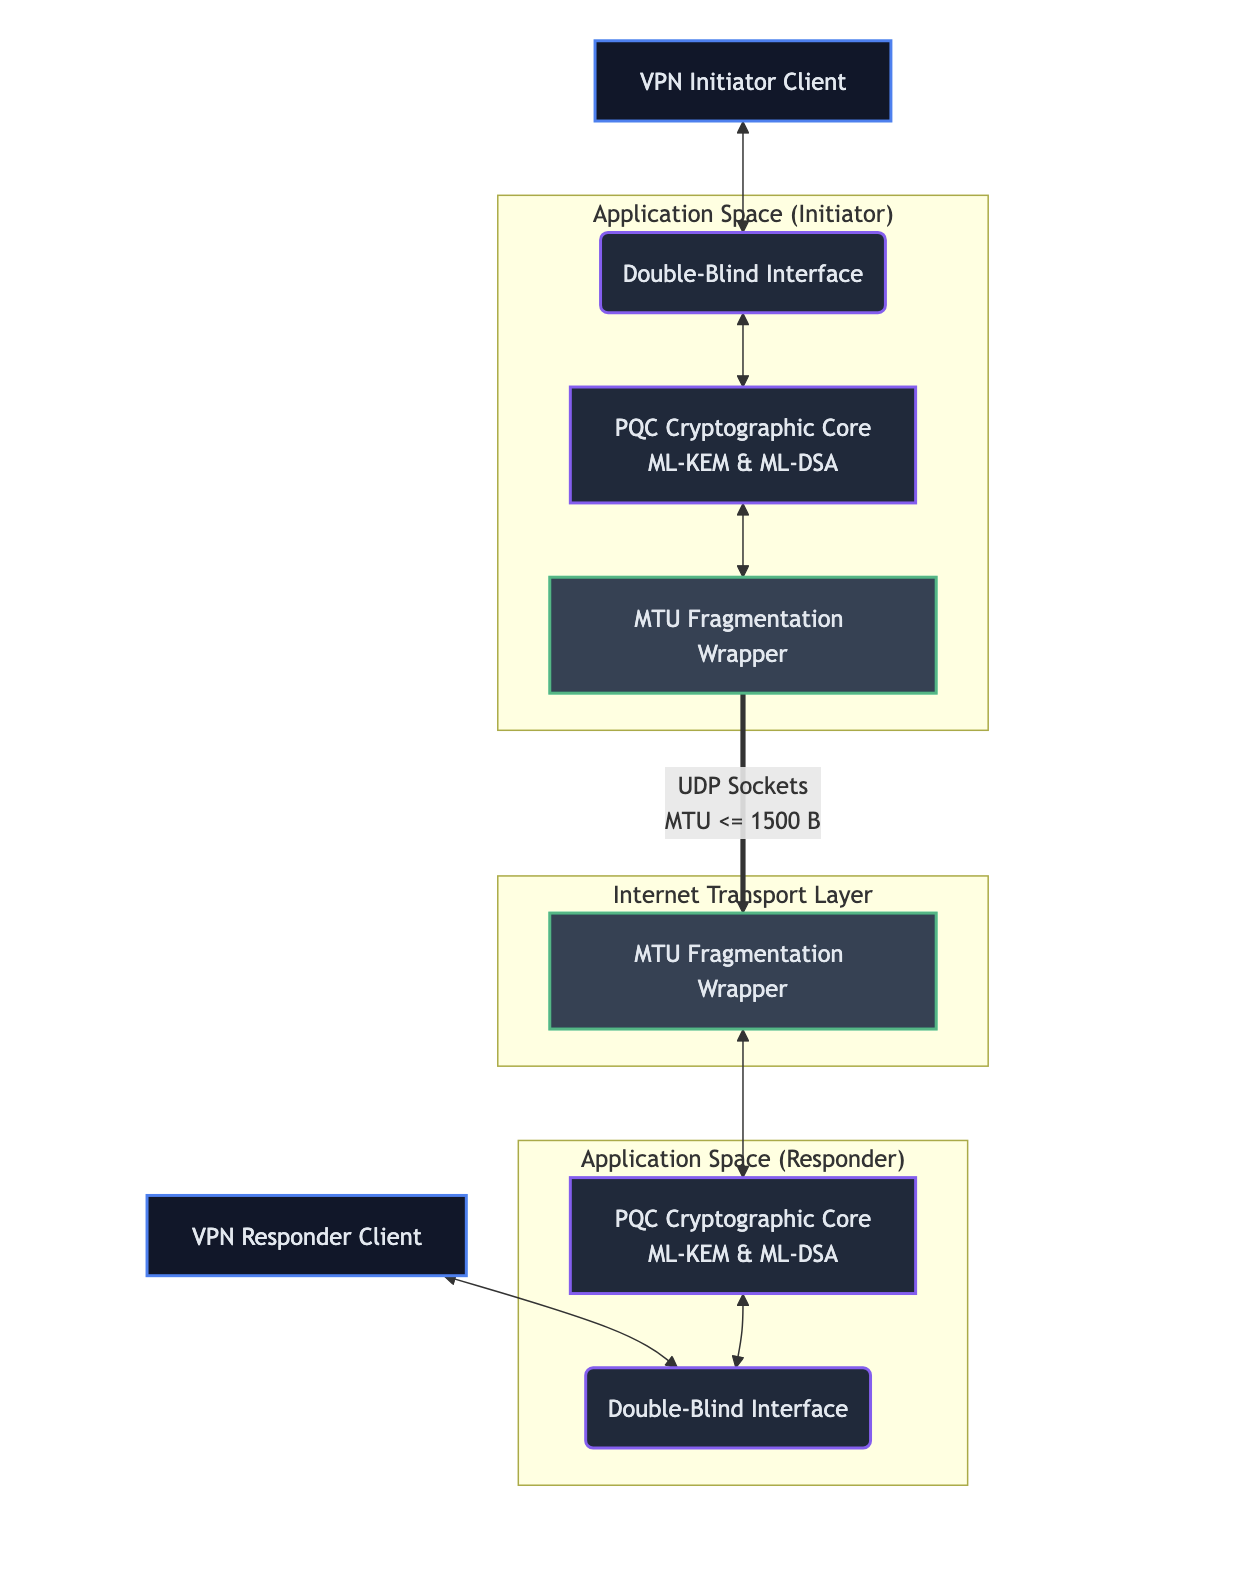
\includegraphics[width=\linewidth]{image.png}
\caption{System architecture showing the separation between application-layer cryptographic operations and kernel-level IP transport.}
\label{fig:architecture}
\end{figure}

The Double-Blind PQC framework employs three cryptographic primitives to achieve a single protocol flow: a lattice-based KEM for key agreement, a lattice-based signature scheme for authentication, and a symmetric-key encryption algorithm for bulk data encryption. This section describes each primitive and the resulting protocol.

\subsection{Cryptographic Primitives}

\textbf{1) ML-KEM-768 (CRYSTALS-Kyber):} ML-KEM-768 serves as the key encapsulation mechanism. Unlike traditional Diffie-Hellman, where an interactive key exchange is performed, KEM-based protocols operate in the following three-step manner:
\begin{enumerate}
    \item \textit{Key Generation}: The Initiator generates its Kyber key pair and publishes the 1,184-byte public key $PK_{KEM}$.
    \item \textit{Encapsulation}: The Responder uses $PK_{KEM}$ to encapsulate the random 32-byte shared secret $SS$, yielding the 1,088-byte ciphertext $CT$.
    \item \textit{Decapsulation}: The Initiator retrieves the shared secret $SS$ using the corresponding private key $SK_{KEM}$.
\end{enumerate}
ML-KEM-768 is designed to achieve a security level equivalent to the AES-192 algorithm. Its performance characteristics, including the efficiency of the key generation phase, show promise compared to the performance of the classical alternatives, as we show in Section~VI.

\textbf{2) ML-DSA-65 (CRYSTALS-Dilithium):} All handshake messages are digitally signed using the ML-DSA-65 digital signature scheme. Dilithium is based on the ``Fiat-Shamir with Aborts'' scheme, which eliminates the threat of information leakage via the signature values. Signature schemes based on lattices were previously vulnerable to this weakness.

However, the cost is high. Dilithium public keys are 1,952 bytes in size, and the signatures are 3,293 bytes. These sizes are one order of magnitude larger than the 32-byte public keys and 64-byte signatures used in Ed25519. These sizes are the main cause of the MTU challenges discussed in Section~V.

\subsection{Handshake Protocol}

The Double-Blind handshake is based on the 1-RTT model. It is assumed that both the Initiator ($I$) and the Responder ($R$) possess pre-provisioned long-term ML-DSA identity key pairs: ($PK_{sig\_I}$, $SK_{sig\_I}$) and ($PK_{sig\_R}$, $SK_{sig\_R}$), respectively.



\textbf{Step 1: Initiation.} $I$ generates its ephemeral ML-KEM-768 key pair ($PK_{kem\_I}$, $SK_{kem\_I}$) and a random 32-byte nonce $Nonce_I$. It signs the concatenation $PK_{kem\_I} \| Nonce_I$ using $SK_{sig\_I}$, then transmits the public key, nonce, and signature to $R$. The fragmentation wrapper (Section~V) splits the payload into UDP packets that are transmitted.

\textbf{Step 2: Validation and Encapsulation.} $R$ reassembles the fragments and verifies the Dilithium signature using $PK_{sig\_I}$. If the signature is invalid, $R$ immediately terminates the connection. Otherwise, $R$ performs KEM encapsulation against $PK_{kem\_I}$ and obtains the shared secret $SS$ and ciphertext $CT$. $R$ signs the combination of $CT$ and $Nonce_R$ using $SK_{sig\_R}$ and sends the response back to $I$ via the fragmentation wrapper.

\textbf{Step 3: Decapsulation.} $I$ reassembles the response and verifies $R$'s signature using $PK_{sig\_R}$ and decapsulates $CT$ to recover $SS$. At this point, both $I$ and $R$ hold the same 32-byte shared secret and the costly asymmetric operations are complete.

\begin{algorithm}[H]
\caption{Double-Blind Handshake \& Encapsulation}\label{alg:handshake}
\begin{algorithmic}[1]
\renewcommand{\algorithmicrequire}{\textbf{Input:}}
\renewcommand{\algorithmicensure}{\textbf{Output:}}
\REQUIRE Initiator ID Key $SK_{I}$, Responder ID Key $PK_{R}$
\ENSURE Local Symmetric Session Array Key $SS_{tunnel}$
\STATE \text{Initialize AES-GCM Transport Pipeline}
\STATE $PK_{KEM}, SK_{KEM} \leftarrow ML\_KEM.GenerateKeyPair()$
\STATE $Nonce_I \leftarrow RandomSecureBitGenerator(32)$
\STATE $Payload_{init} \leftarrow (PK_{KEM} || Nonce_I)$
\STATE $Signature_{init} \leftarrow ML\_DSA.Sign(SK_{I}, Payload_{init})$
\STATE $TransmitArray(Payload_{init} || Signature_{init})$
\WHILE{System Wait For Responder Feedback}
    \STATE $Payload_{resp}, Signature_{resp} \leftarrow ReceiveArray()$
    \IF{$!ML\_DSA.Verify(PK_{R}, Payload_{resp}, Signature_{resp})$}
        \STATE \textbf{return} $CONNECTION\_REJECTED\_FATAL$
    \ENDIF
    \STATE $CT_{KEM}, Nonce_R \leftarrow ParseObject(Payload_{resp})$
    \STATE $SS_{tunnel} \leftarrow ML\_KEM.Decapsulate(SK_{KEM}, CT_{KEM})$
    \STATE \textbf{break}
\ENDWHILE
\STATE \textbf{return} $SS_{tunnel}$
\end{algorithmic}
\end{algorithm}

\subsection{Symmetric Tunnel Establishment}
After the completion of the handshake, the shared secret $SS$ is available. The costly asymmetric operations are complete. The raw 32-byte secret is then expanded to create a 256-bit symmetric key through the Key Derivation Function BLAKE2s. This 256-bit symmetric key is then used to create an \textbf{AES-256-GCM} (Galois/Counter Mode) tunnel for all the data traffic. AES-256 is secure against Grover's attack, which requires 128 bits of security, considered sufficient for the foreseeable future \cite{nist2022pqc}.

\begin{figure}[!t]
\centering
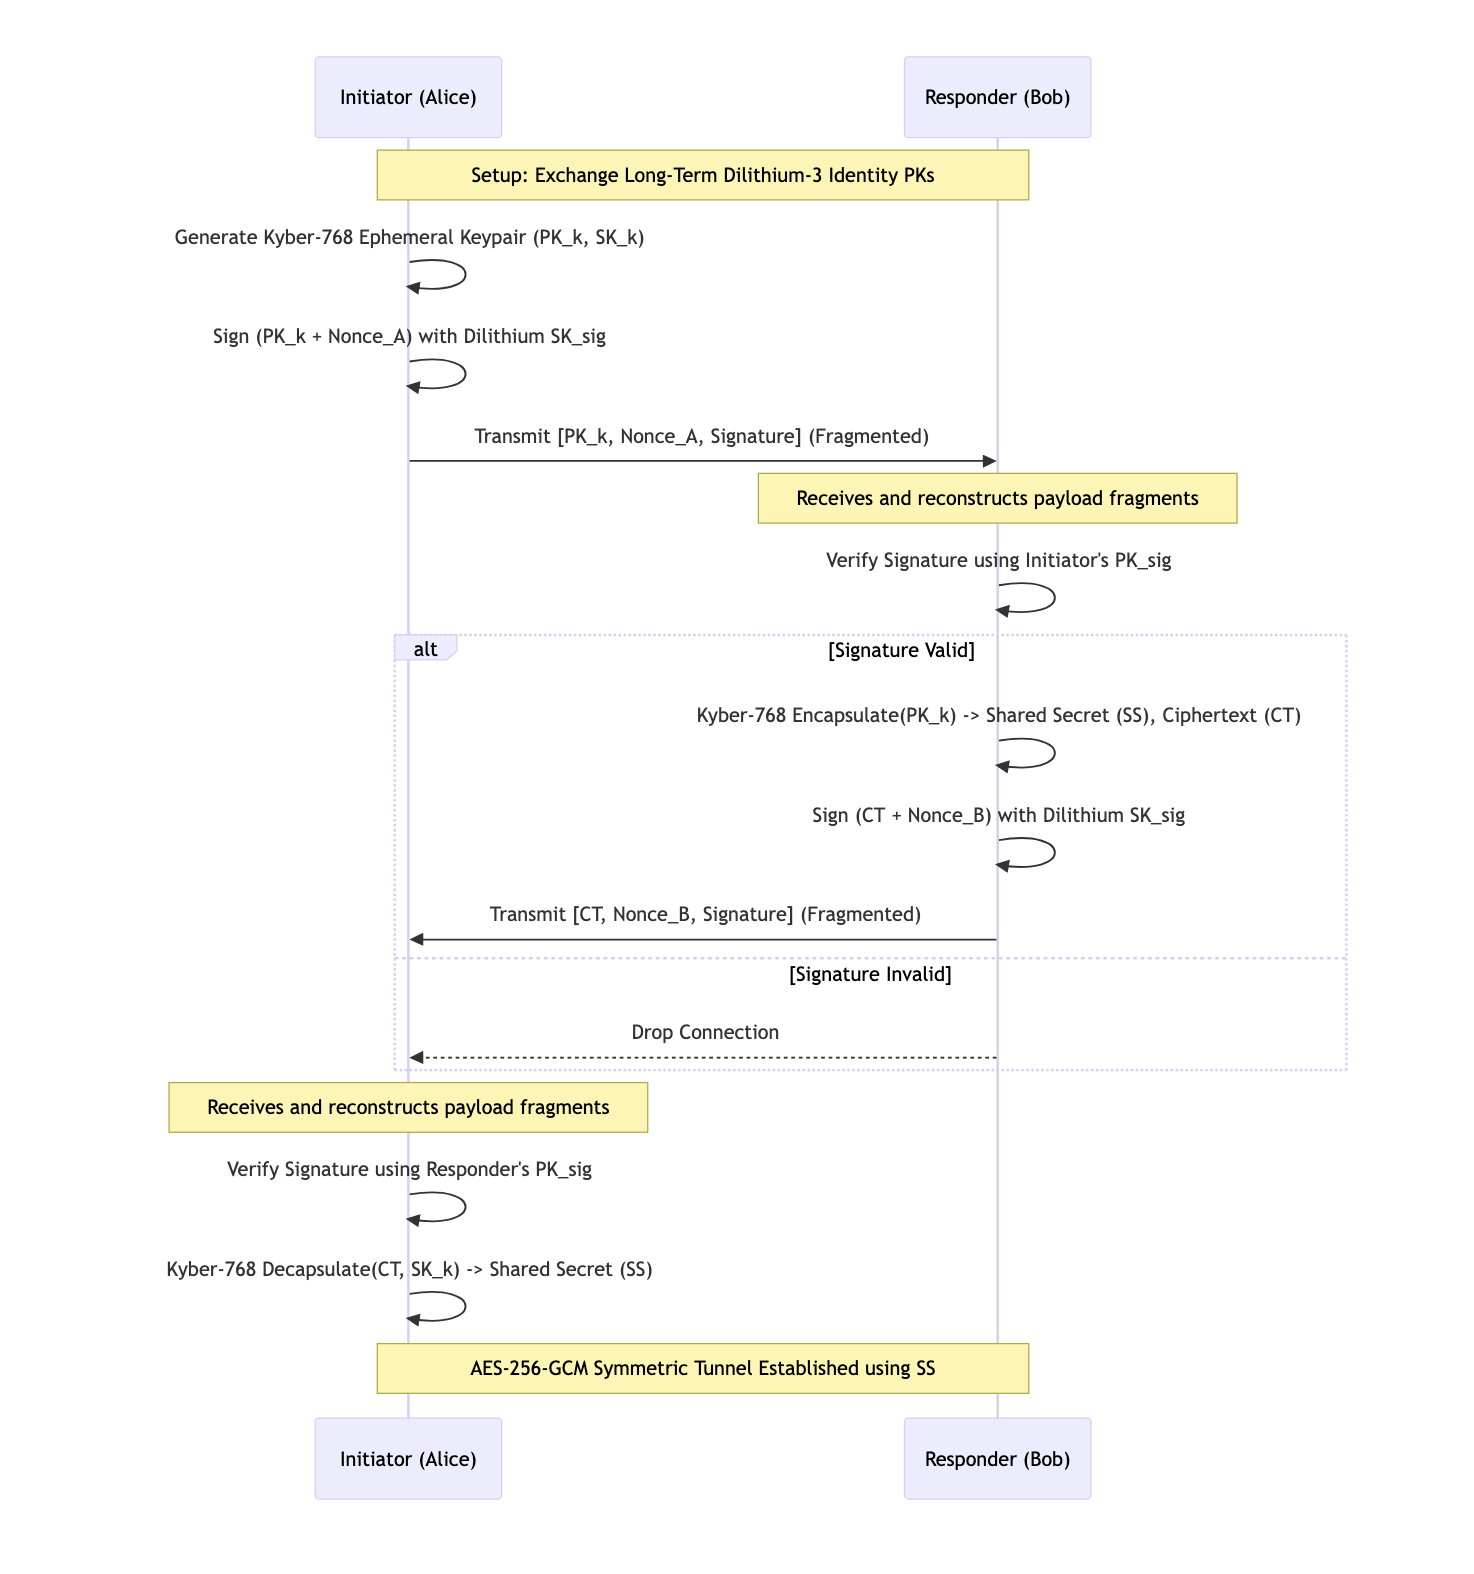
\includegraphics[width=\linewidth]{image2.png}
\caption{Sequence diagram of the Double-Blind PQC handshake protocol.}
\label{fig:sequence}
\end{figure}


\section{Network Engineering: Application-Layer Fragmentation}
The large size of the keys and signatures of post-quantum algorithms presents a transport problem that must be addressed before any PQC VPN can function. The following sections describe the problem and the solution.

\subsection{The MTU Problem}
The maximum size of a single Ethernet frame is 1,500 bytes. If we then account for IP and UDP headers, which sum to 28 bytes in total, then the payload of each datagram is approximately 1,472 bytes. If we then calculate the size of a single Double-Blind handshake message - consisting of a Kyber key, a Dilithium signature, and a one-time nonce - we get approximately 4,500 bytes, which is far in excess of the payload of a single datagram.

If this large payload is sent to the OS kernel, then the kernel will fragment this datagram into multiple IP fragments. If this datagram is then sent over UDP, this is unreliable: the loss of any single fragment means the entire message is effectively lost, with no fall-back mechanism for retransmitting the missing fragments. On congested or lossy networks, this makes handshake completion unpredictable and can prevent tunnel establishment.

\subsection{Deterministic Application-Layer Fragmentation}
To avoid the OS layer fragmentation issue entirely, we also implemented a \textbf{Fragmentation Wrapper} at the application layer. Before writing the data to the UDP socket, the wrapper splits the data into smaller chunks, where each chunk is no longer than \texttt{CHUNK\_SIZE} bytes. \texttt{CHUNK\_SIZE} is set to 1,000 by default, leaving some buffer room below the MTU.

Each piece of the data is prefixed with a small 6-byte header:
\begin{itemize}
    \item \texttt{Message\_ID} (2 bytes): It is like a special code, a random 16-bit identifier.
    \item \texttt{Fragment\_Index} (2 bytes): The sequential index of the fragment.
    \item \texttt{Total\_Fragments} (2 bytes): The total number of fragments.
\end{itemize}

The fragmentation process is shown in Algorithm~\ref{alg:frag}.

\begin{algorithm}[H]
\caption{Deterministic MTU Payload Extractor}\label{alg:frag}
\begin{algorithmic}[1]
\REQUIRE Encrypted Monolithic Payload $P_{enc}$, Defined $MTU_{limit}$
\ENSURE Sequential List of Compliant UDP Packets $U$
\STATE $L \leftarrow ByteLength(P_{enc})$
\IF{$L \leq MTU_{limit}$}
    \STATE $Header \leftarrow (RandomUInt16() || 0 || 1)$
    \STATE $Transmit(Header || P_{enc})$
    \STATE \textbf{return} 1
\ENDIF
\STATE $N \leftarrow \lceil L / MTU_{limit} \rceil$
\STATE $SessionID \leftarrow RandomUInt16()$
\STATE $U \leftarrow []$
\FOR{$i = 0$ to $N - 1$}
    \STATE $StartBoundary \leftarrow i \times MTU_{limit}$
    \STATE $EndBoundary \leftarrow Minimum((i + 1) \times MTU_{limit}, L)$
    \STATE $ChunkData \leftarrow P_{enc}[StartBoundary : EndBoundary]$
    \STATE $Header \leftarrow (SessionID || i || N)$
    \STATE $U[i] \leftarrow (Header || ChunkData)$
    \STATE $Socket.SendTo(U[i])$
\ENDFOR
\STATE \textbf{return} $N$
\end{algorithmic}
\end{algorithm}

\begin{figure}[!t]
\centering
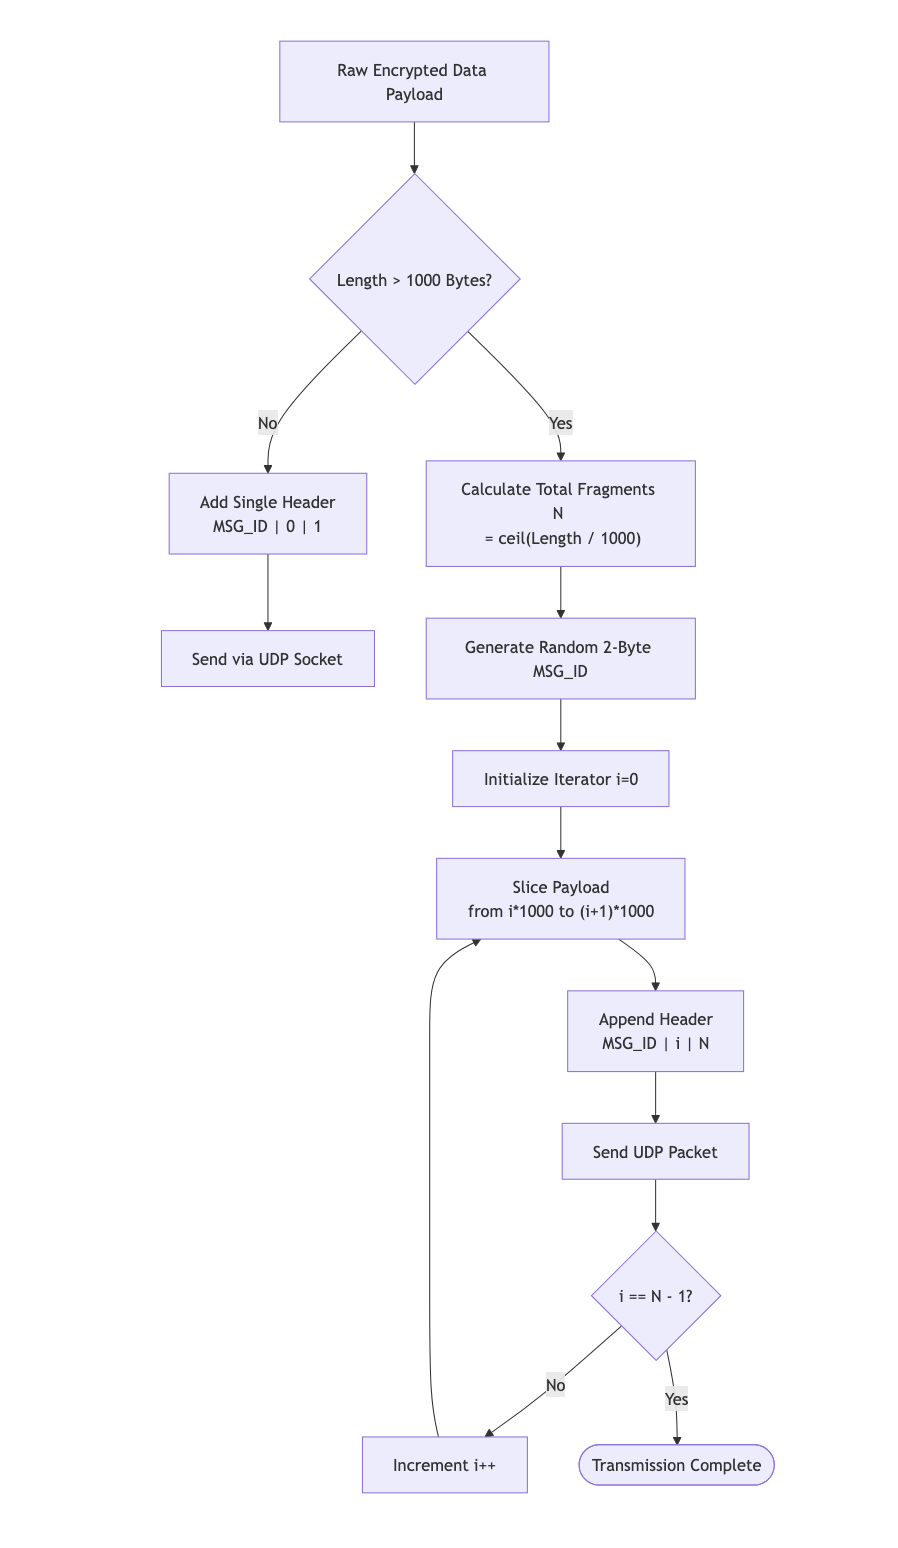
\includegraphics[width=\linewidth]{image3.png}
\caption{Flowchart of the application-layer fragmentation logic.}
\label{fig:fragmentation}
\end{figure}

\subsection{Reassembly and Timeout Handling}
On the receiver side, fragments are buffered in a dictionary using \texttt{Message\_ID} as a key. Upon receiving fragments, which may not necessarily arrive in order due to the unordered nature of UDP, they are placed in their correct order based on \texttt{Fragment\_Index}. Once all fragments for a particular \texttt{Message\_ID} are received, which is a total of $N$ fragments, the buffer is simplified to a more manageable format and the original information is sent to the cryptographic layer for processing.

To prevent memory exhaustion from incomplete or malicious fragment streams, the reassembly engine enforces a configurable timeout. If all fragments for a given message are not received within the time limit, only the partial information gets through and is discarded, and the handshake layer may request retransmission. This provides basic resilience against both network instability and denial-of-service attacks targeting the fragment buffer.


\section{Experimental Setup and Performance Analysis}
To evaluate the computational overhead imposed by the Double-Blind PQC framework, a benchmarking study was conducted comparing our post-quantum primitives with widely used classical algorithms. Our goal was to quantify the practical trade-offs associated with using PQC in a VPN.

\subsection{Methodology}
The benchmarking suite was integrated with the application's Python backend and executed locally to minimize variance in network latency while measuring cryptographic computation times. We used Python's \texttt{time.perf\_counter()} for high-resolution timing. We performed 25 iterations of the algorithm, and the results are based on $N = 25$ iterations, which provide arithmetic means. This number of iterations is sufficient to average out variations in operating system scheduling jitter while keeping benchmark execution times reasonable.

The following are the classical algorithms used as a reference in this work:
\begin{itemize}
    \item \textbf{X25519 (ECDH)}: Elliptic curve used in WireGuard. This represents the current state of the art in VPN key exchange algorithms.
    \item \textbf{SECP256R1 (P-256)}: NIST standard elliptic curve. This is a standard elliptic curve used in TLS and corporate VPNs.
    \item \textbf{Ed25519}: High-performance signature scheme using Edwards curves, which is commonly used in SSH and code signatures.
    \item \textbf{RSA-3072 / RSA-PSS}: Traditional integer factorization algorithms.
\end{itemize}

\subsection{Key Encapsulation Results}
Table~\ref{tab:kem} lists key generation and encapsulation/exchange latencies for each KEM or key agreement algorithm.

\begin{table}[hbt!]
\centering
\caption{KEM / Key Exchange Performance (mean of 25 iterations)}
\label{tab:kem}
\resizebox{\columnwidth}{!}{
\begin{tabular}{l c c c c}
\toprule
\textbf{Algorithm} & \textbf{KeyGen (ms)} & \textbf{Exch/Encap (ms)} & \textbf{Pub Key (B)} \\
\midrule
ML-KEM/Kyber-768 & 0.063 & 0.081 & 1184 \\
X25519 (ECDH) & 0.174 & 0.235 & 32 \\
P-256 (SECP256R1) & 0.355 & 0.442 & 65 \\
RSA-OAEP (3072-bit) & 240.150 & 0.812 & 384 \\
\bottomrule
\end{tabular}
}
\end{table}

The results are striking. ML-KEM-768 achieves key generation in 0.063~ms - roughly 2.8$\times$ faster than X25519 (0.174~ms). It's significantly faster, at 5.6 times the speed of P-256 (0.355~ms), and nearly 3,800$\times$ faster than RSA-3072 (240.150~ms). The encapsulation step is similarly fast at 0.081~ms, outperforming all classical alternatives.

These numbers may seem counterintuitive: how can a post-quantum algorithm with larger keys be faster than ECC? The answer lies in the underlying arithmetic. Kyber's operations consist primarily of polynomial multiplications over small modular rings, which map efficiently to CPU instructions. Elliptic curve operations, by contrast, require expensive modular exponentiation, and RSA key generation involves searching for large primes - an inherently slow operation.

The trade-off, as discussed in Section~III, is key size. The key size of Kyber's 1,184-byte public key is much larger, 37 times larger, compared to the 32-byte key size of X25519. For establishing a VPN, creating a single tunnel is a one-time operation. The operation is handled transparently by the fragmentation wrapper. The overall impact is that adopting PQC actually decreases handshake computation time. In addition, there is a small increase in network bandwidth required for establishing the tunnel.

\subsection{Digital Signature Results}
Table~\ref{tab:sig} illustrates the performance of each digital signature scheme in terms of sign, verify, and size.

\begin{table}[hbt!]
\centering
\caption{Digital Signature Performance (mean of 25 iterations)}
\label{tab:sig}
\resizebox{\columnwidth}{!}{
\begin{tabular}{l c c c }
\toprule
\textbf{Algorithm} & \textbf{Sign (ms)} & \textbf{Verify (ms)} & \textbf{Sig Size (B)} \\
\midrule
ML-DSA/Dilithium-3 & 0.124 & 0.041 & 3293 \\
Ed25519 & 0.092 & 0.210 & 64 \\
ECDSA (P-256) & 0.184 & 0.362 & 71 \\
RSA-PSS (3072-bit) & 3.420 & 0.105 & 384 \\
\bottomrule
\end{tabular}
}
\end{table}

While the signing time for Dilithium is slightly longer at 0.124~ms, compared to Ed25519's 0.092~ms, the verification time for Dilithium is about 5 times faster at 0.041~ms. In the context of a VPN, the verification time is more important than the signing time, as the responding party must verify the signatures before proceeding with the handshake. In comparison to ECDSA, which takes 0.362~ms to verify, and RSA-PSS, which takes 0.105~ms, the verification time for Dilithium is the fastest among the tested methods.

As with the previous methods, the cost is in the size, with Dilithium signatures measuring 3,293 bytes. In comparison to Ed25519, which requires 64 bytes, this is a whopping 51 times increase. This is the largest contributor to the MTU challenges discussed in Section~V.

\section{Conclusion and Future Work}
In the above paper, the reader has been introduced to Double-Blind PQC, an application layer-based system for integrating NIST's PQC standards into the VPN infrastructure. The system uses ML-KEM-768 for key encapsulation, ML-DSA-65 for authentication, and a deterministic wrapper to connect the two.

As the above benchmarks demonstrate, the computational cost of PQC is not an issue; ML-KEM-768's key generation is faster than all the tested classical alternatives, while Dilithium-3's signature verification is the fastest. The cost is in the bandwidth; the increased size requires careful engineering to ensure the PQC is properly transported. This is exactly what the wrapper does.

There are a number of avenues for further work. One is to port the cryptographic core from Python to a language like Rust or C, which would help reduce latency per operation and would help to further characterize the performance limit of this method. Second, integration with hybrid protocols, which include both classical and quantum-resistant algorithms (such as X25519 and Kyber), would add a layer of protection during this transition phase. Third, formal verification of the handshake protocol by tools such as ProVerif or Tamarin would further increase confidence in the security benefits. Finally, in addition to testing in a lab environment, testing in a variety of different network environments, such as those involving high latency satellite networks or lossy mobile networks, would validate the performance of the fragmentation wrapper.

\begin{thebibliography}{00}
\bibitem{hulsing2017pqwireguard} A. H\"ulsing, K.-C. Ning, P. Schwabe, F. J. Weber, and P. R. Zimmermann, ``Post-quantum WireGuard,'' \textit{Eindhoven University of Technology, Max Planck Institute, Radboud University}, 2017.
\bibitem{shim2025qtrustnet} H. Shim, B. Kang, H. Im, D. Jeon, and S.-M. Kim, ``qTrustNet Virtual Private Network (VPN): Enhancing Security in the Quantum Era,'' \textit{IEEE Access}, vol. 13, Jan. 2025. 
\bibitem{nist2022pqc} National Institute of Standards and Technology (NIST), ``Post-Quantum Cryptography Standardization,'' 2022.
\end{thebibliography}

\end{document}
